\documentclass{beamer}
\usetheme{CENIDETDIE}
\setbeamertemplate{caption}[numbered]
\usefonttheme[onlymath]{serif}

% ------------------------------------------------------------------------------------------------

\usepackage[utf8]{inputenc}
\usepackage[T1]{fontenc}
\usepackage{helvet}
\usepackage{graphicx} % Allows including images
\usepackage{booktabs} % Allows the use of \toprule, \midrule and \bottomrule tables
\usepackage{amsmath}
\usepackage{color}
\usepackage{hyperref}
\usepackage{subfig}
\usepackage[document]{ragged2e}
%\usepackage{authblk} %many authors
\numberwithin{figure}{section}
%\numberwithin{equation}{section}
\usepackage{natbib}

% ------------------------------------------------------------------------------------------------

\title{\textbf{ \textit{W+jets to Leptons}}}
%\subtitle{{\small }}
\author[C.Salazar]{\textbf{Camilo A Salazar G} }
\institute[UdeA]{camilo.salazar@cern.ch}

%\author{\textit{\textbf{Camilo A Salazar G}}}
%\institute{\url{camilo.salazar@cern.ch} }
\date{\today}


% ------------------------------------------------------------------------------------------------

\begin{document}

% ------------------------------------------------------------------------------------------------

\begin{frame}[plain,t]
\titlepage
\end{frame}


% ------------------------------------------------------------------------------------------------

\begin{frame}[plain,noframenumbering]
  \addtocounter{framenumber}{-1}
  \scriptsize
%   \thispagestyle{empty}
  \frametitle{Contenido}
  \setbeamertemplate{section in toc}[sections numbered]
  \tableofcontents[hideallsubsections]
\end{frame}

% ------------------------------------------------------------------------------------------------

\section{Introducción}

\begin{frame}
    \frametitle{Introducción}
    \justifying{}
    
    \begin{itemize}
        \item[]
        \item[] Processes under study:
        \begin{enumerate}
            \item Z+Jets.
            \item W+Jets.
        \end{enumerate}
    \end{itemize}


\end{frame}

% ------------------------------------------------------------------------------------------------

\section{Últimos Resultados}
\begin{frame}
 \frametitle{Latest Results}
 \justifying{The results }
 
 
 \begin{itemize}
    \item[] 
    \item[] Validation:
    \begin{itemize}
         \item Rivet validate against data samples.
        \item Validate against MG+pythia8 samples.
     \end{itemize}
 \end{itemize} 
 
\end{frame}

% ------------------------------------------------------------------------------------------------

\section{Herwig 7 generation in CMSSW\_10\_2\_6}
\begin{frame}
 \frametitle{Herwig 7 generation in CMSSW\_10\_2\_6}
    \justifying{Herwig have some matrix element build in, and also have support for some external LO and NLO matrix element(ME) providers, and also several showers }
\vspace{25px}

 \begin{columns}[c] % The "c" option specifies centered vertical alignment while the "t" option is used for top vertical alignment

 \column{.4\textwidth} % Left column and width
    
    \large{\textbf{ME}}
    \footnotesize
    \begin{itemize}
        \item MadGraph-GoSam
        \item MadGraph-MadGraph
        \item MadGraph-OpenLoops
        \item MadGraph-NJet
        \item HJets
        \item VBFNLO
    \end{itemize}

 \column{.6\textwidth} % Right column and width
    \large{\textbf{Matching and shower}}
    \footnotesize
    \begin{itemize}
        \item MCat[LO-NLO]-[Default-DipoleShower]Shower    
        \item Powheg-[Default-DipoleShower]Shower
        \item LO-[Default-DipoleShower]Shower
        \item .[LO-NLO]-NoShower

    \end{itemize}
 \end{columns}

\end{frame}

% -------------------------------------------------------------

\subsection{Build in}
\begin{frame}
 \frametitle{Build in,  $p p \rightarrow  W+Jets$ and  $p p \rightarrow  Z+Jest$}
 
    \begin{figure}
        \centering
        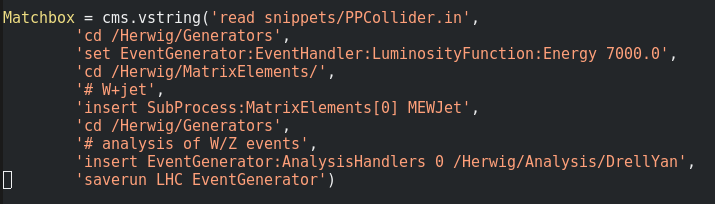
\includegraphics[width=\textwidth]{pictures/WJetsBuildIn}
    \end{figure}
 
    \begin{exampleblock}{In the similar way it is the $p p \rightarrow  Z$ process.}
        \url{https://github.com/casfisica/Herwig7-Interface/blob/master/Herwig7_ppToW_Build_In.py}
    \end{exampleblock}
 
\end{frame}



% -------------------------------------------------------------

\subsection{External ME providers}
\begin{frame}
 \frametitle{External ME providers}
     \begin{figure}
    \centering
    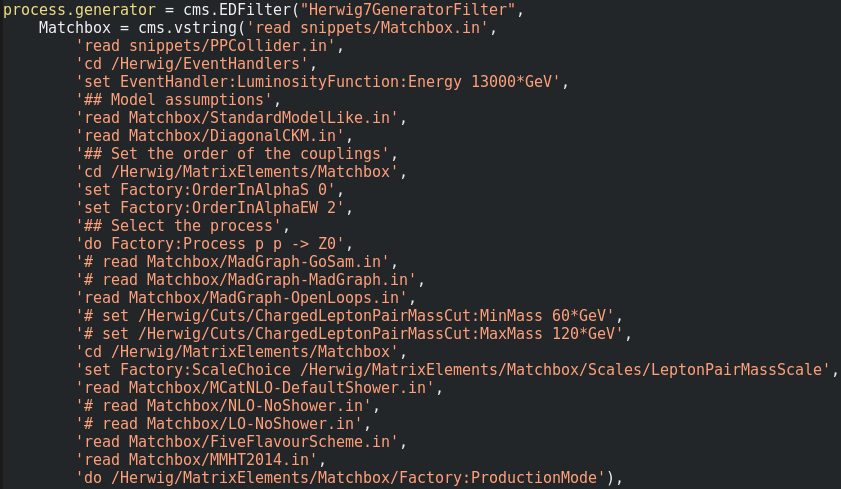
\includegraphics[width=\textwidth]{pictures/ConfigZ0}
    \end{figure}

\begin{exampleblock}{Generate events using CMSSW}
\url{https://github.com/casfisica/Herwig7-Interface/blob/master/Herwig7_Matchbox_90X_ppToW_GEN_SIM.py}
 \end{exampleblock}

\end{frame}


% -------------------------------------------------------------

\section{Rivet Interface}
\begin{frame}
\frametitle{Rivet Interface}
 The Rivet package can be used directly from Herwig
 
 \begin{figure}
  \centering
  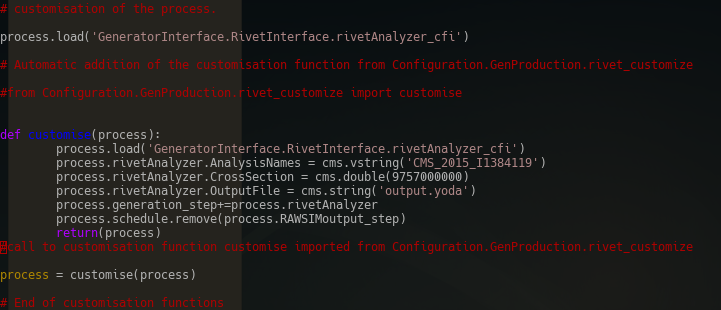
\includegraphics[width=\textwidth]{pictures/Rivet}
 \end{figure}
 
 \begin{exampleblock}{CMSSW create a Yoda file}
     \small{}  
 \end{exampleblock}

\end{frame}


% -------------------------------------------------------------


\section{Results}
\subsection{W+Jets}
\begin{frame}
 \frametitle{Results: $W+Jets$} 

\begin{figure}[!tbp]
  \centering
  \subfloat[]{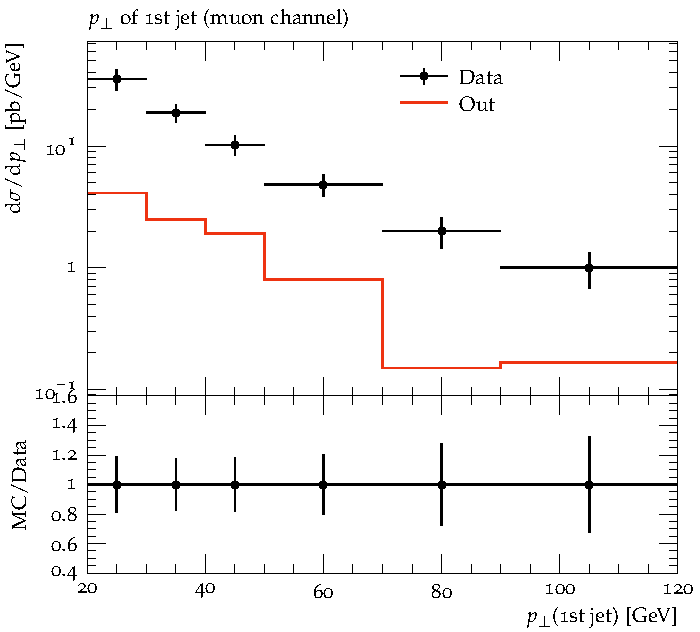
\includegraphics[width=0.5\textwidth]{pictures/ATLAS_2010_S8919674_d06-x01-y01_WBI}\label{fig:f1}}
  \hfill
  \subfloat[]{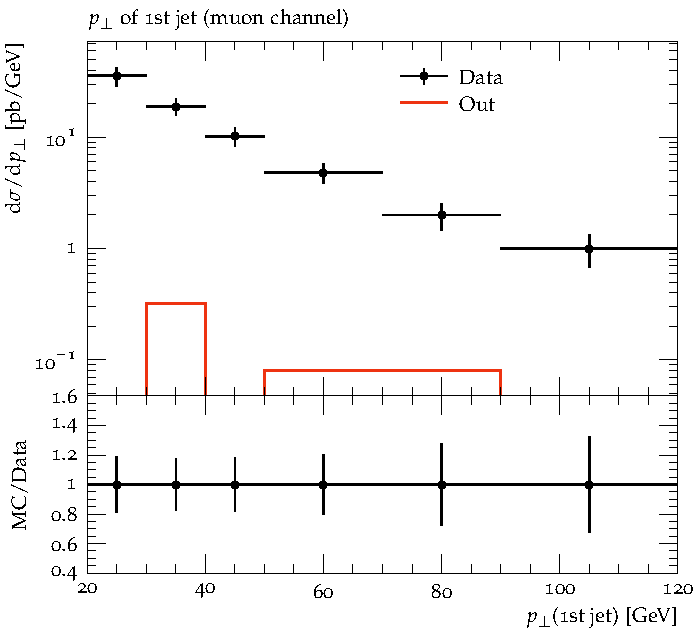
\includegraphics[width=0.5\textwidth]{pictures/ATLAS_2010_S8919674_d06-x01-y01_WMB}\label{fig:f2}}
  \caption{\scriptsize{ATLAS (7 TeV) $W+Jets$ cross-section as a function of the $p_T$ of the leading jet in the even. Comparison between Build-In (a) and MadGraph-OpenLoops (b) ME,  Eur.Phys.J. C75 (2015) 82, doi:10.1140/epjc/s10052-015-3262-7, arXiv:1409.8639 [hep-ex]}}
\end{figure}
 

\end{frame}

% ----------------------------------------------------------------


\begin{frame}
 \frametitle{Results: $W+Jets$} 

\begin{figure}[!tbp]
  \centering
  \subfloat[]{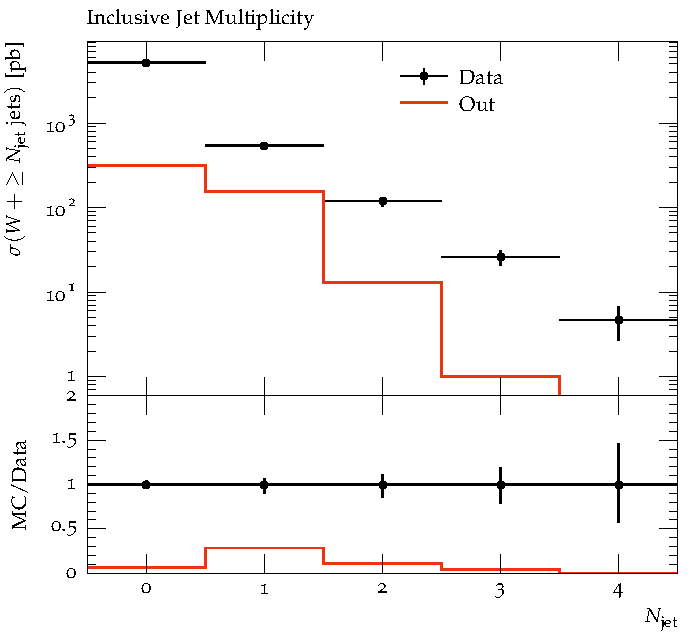
\includegraphics[width=0.5\textwidth]{pictures/ATLAS_2012_I1083318_d01-x01-y01_WBI}\label{fig:f1}}
  \hfill
  \subfloat[]{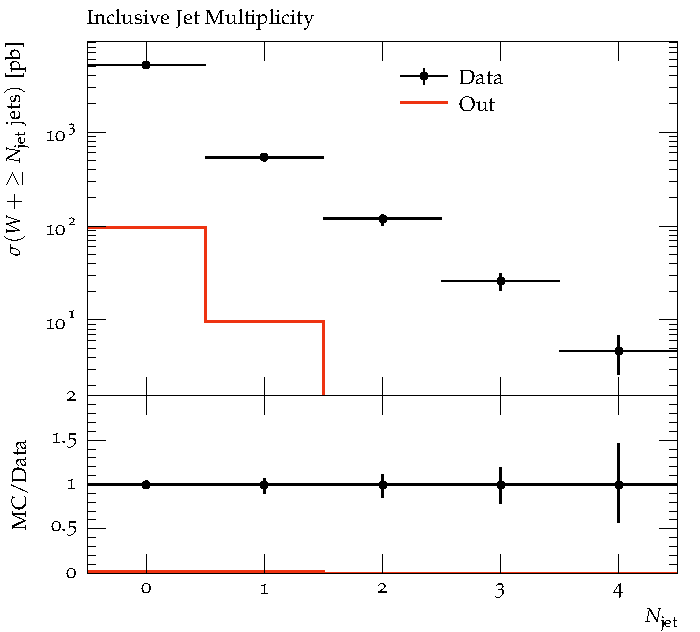
\includegraphics[width=0.5\textwidth]{pictures/ATLAS_2012_I1083318_d01-x01-y01_WMB}\label{fig:f2}}
  \caption{\scriptsize{ATLAS (7 TeV) $W+jets$ cross section results as a function of corrected jet multiplicity. Comparison between Build-In (a) and MadGraph-OpenLoops (b) ME, arXiv:1201.1276}}
\end{figure}
 

\end{frame}

% ----------------------------------------------------------------


\begin{frame}
 \frametitle{Results: $W+Jets$} 

\begin{figure}[!tbp]
  \centering
  \subfloat[]{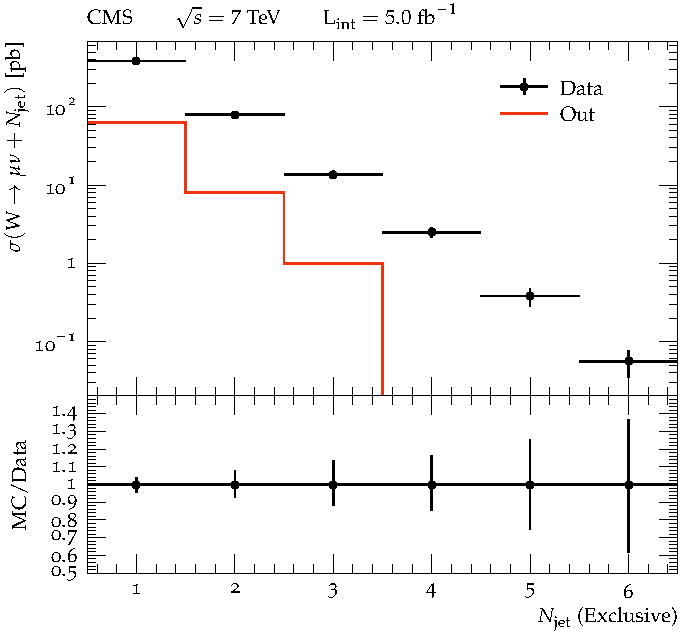
\includegraphics[width=0.5\textwidth]{pictures/CMS_2014_I1303894_d13-x01-y01_WBI}\label{fig:f1}}
  \hfill
  \subfloat[]{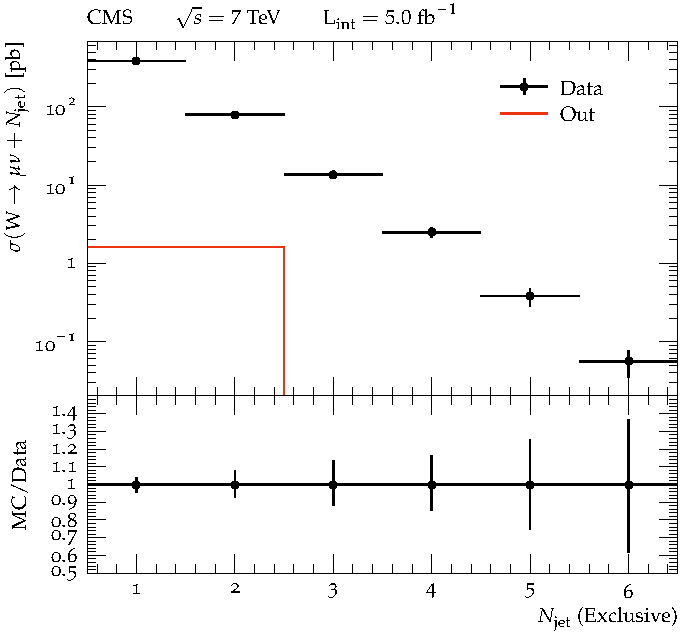
\includegraphics[width=0.5\textwidth]{pictures/CMS_2014_I1303894_d13-x01-y01_WMB}\label{fig:f2}}
  \caption{\scriptsize{CMS (7 TeV) $W+jets$ cross section results as a function of jet multiplicity. Comparison between Build-In (a) and MadGraph-OpenLoops (b) ME, arXiv:1303.4811}}
\end{figure}
 

\end{frame}

% -------------------------------------------------------------


\subsection{Z+Jets}
\begin{frame}
 \frametitle{Results: $Z+Jets$} 

\begin{figure}[!tbp]
  \centering
  \subfloat[]{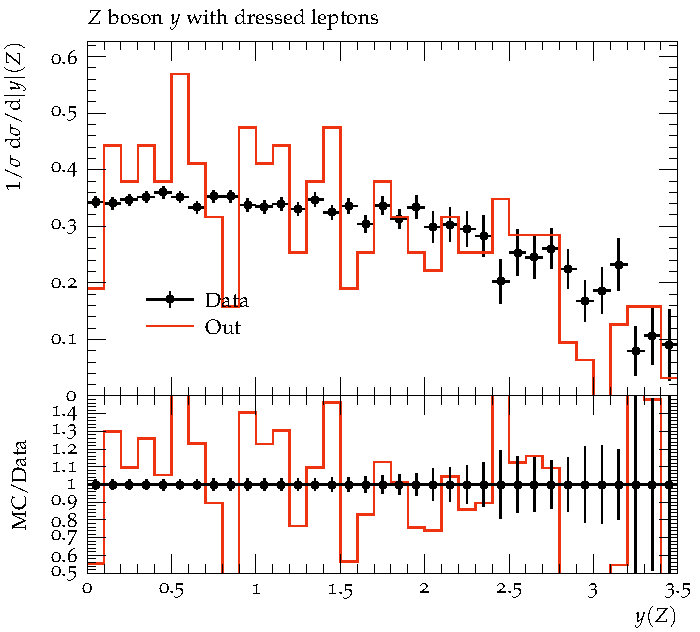
\includegraphics[width=0.5\textwidth]{pictures/CMS_2012_I941555_d01-x01-y03_ZBI}\label{fig:f1}}
  \hfill
  \subfloat[]{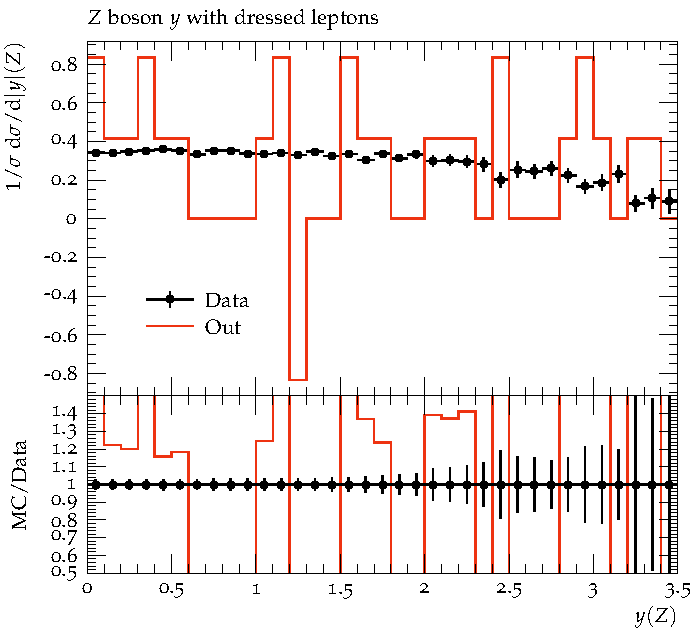
\includegraphics[width=0.5\textwidth]{pictures/CMS_2012_I941555_d01-x01-y03_ZMB}\label{fig:f2}}
  \caption{\scriptsize{CMS (7 TeV) The normalized differential cross section for Z bosons as a function of the absolute value of rapidity. Comparison between Build-In (a) and MadGraph-OpenLoops (b) ME,  Phys.Rev. D85 (2012) 032002, arXiv:1110.4973, CMS-EWK-10-010, CERN-PH-EP-2011-169}}
\end{figure}
 

\end{frame}

% ----------------------------------------------------------------

\begin{frame}
 \frametitle{Results: $Z+Jets$} 

\begin{figure}[!tbp]
  \centering
  \subfloat[]{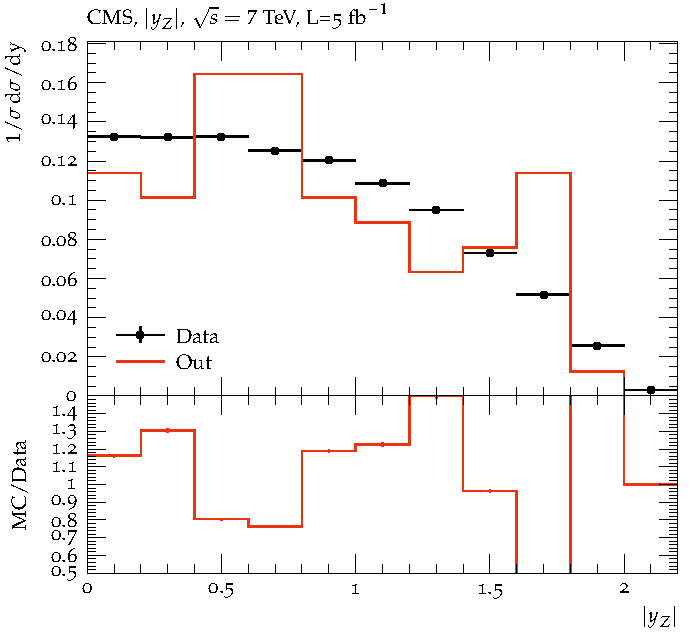
\includegraphics[width=0.5\textwidth]{pictures/CMS_2013_I1258128_d01-x01-y01_ZBI}\label{fig:f1}}
  \hfill
  \subfloat[]{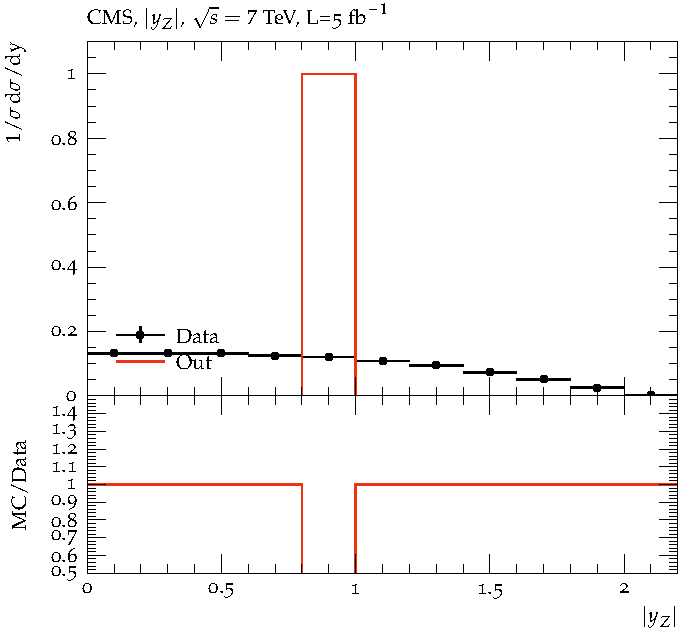
\includegraphics[width=0.5\textwidth]{pictures/CMS_2013_I1258128_d01-x01-y01_ZMB}\label{fig:f2}}
  \caption{\scriptsize{CMS (7 TeV) Distributions in absolute values of rapidities for $Z+ 1 Jet$ normalized to unity. .Comparison between Build-In (a) and MadGraph-OpenLoops (b) ME, arXiv:1310.3082}}
\end{figure}
 

\end{frame}
% ----------------------------------------------------------------


\section{Summary}
\begin{frame}
 \frametitle{Summary}
    \begin{itemize}
        \item We produce a $pp \rightarrow Z+Jets$ and $pp \rightarrow W^\pm +Jets$ samples using:
        \begin{itemize}
            \item Build-in ME.
            \item MadGraph-OpenLoops.
        \end{itemize}
    
    \item Use Rivet to compare the H7 MC events to data at 7 TeV, from ATLAS and CMS.
    \item MadGraph-OpenLoops ME, in general, shows a different behavior than Build-In ME.
    
    \end{itemize}
    
    
    \centering{Many thanks to \textbf{Andrej} for your help.}
    
\end{frame}
% ----------------------------------------------------------------

\section{Present issues  and TDL}
\begin{frame}
 \frametitle{Present issues and to do list}
 \textbf{Present issues}
 
 \begin{itemize}
    \item Not able to produce events using MadGraph-MadGraph nor MadGraph-NJet ME.
    \item Differences between MadGraph-OpenLoops ME and Build-In ME.
  \end{itemize}
  
 \textbf{To do list}
    \begin{itemize}
        \item Condor scripts.
        \item Others external ME.
        \item Go to 13TeV.
        \item Compare to MadGraph-Pythia8.
 \end{itemize}


\end{frame}



%\begin{frame}[fragile] % Need to use the fragile option when %verbatim is used in the slide
%\frametitle{Citation}
%An example of the \verb|\citep| command to cite within the %presentation:\\~%
%
%This statement requires citation \citep{skogestad2003simple}.
%\end{frame}

% ------------------------------------------------------------------------------------------------

%\begin{frame}[allowframebreaks]{References}
 %\setbeamertemplate{bibliography item}[text]
 %\bibliographystyle{apalike}
 %\bibliography{references.bib}{}
%\end{frame}

% ------------------------------------------------------------------------------------------------

\ThankYouFrame

% ------------------------------------------------------------------------------------------------

\end{document}
